\documentclass[twocolumn]{article}
\usepackage[utf8]{inputenc}

\usepackage[backend=bibtex,style=ieee]{biblatex}
\bibliography{biblio_dvs_emu_paper}

\usepackage{graphicx}
\graphicspath{{./pictures/}}

\usepackage{amsmath}

%\usepackage{multicol}

%opening
\title{A Real-time Dynamic Vision Sensor Emulator using Off-the-shelf Hardware}
\author{Pineda García, Garibaldi \and Camilleri, Patrick \and Furber, Steve}



\begin{document}

\maketitle
%\begin{multicols}{2}
%[
\begin{abstract}
\textsf{Vision is one of our most important senses, a vast amount of information is perceived through our eyes. Neuroscientists have performed several studies using vision as input to their experiments. However, computational neuroscience has typically used Poisson-encoded images as spike-based visual sources. Recently neuromorphic Dynamic Vision Sensors have surfaced, while they have excellent capabilities, they remain scarce and difficult to use.}


\textsf{
We propose a visual input system inspired by the behaviour of a DVS, but using a digital camera as a sensor. By using readily-available components, we believe, most scientist would have access to a spiking visual input source. While the primary goal was to use the system as a real-time input, it is also able to transcode well established images and video databases into spike train representations. Our main contributions are adding locally inhibitory behaviour, adaptive thresholds and proposing time-based encoding of the output spikes.}

\end{abstract}
%]

\section{Introduction}

In recent years the performance of computer processors has been advancing in smaller increments than it used to a few years ago. This is mainly because manufacturing technologies are reaching their limits. One way to improve performance is to use many processors in parallel, which has been successfully applied to parallel-friendly applications like computer graphics. Task like pattern recognition are still a hard task for computers even with these technological advances.

Our brains are particularly good at learning and recognizing visual patterns (e.g. letters, dogs, houses, etc.). In order to achieve better performance for similar tasks on computers, scientists have looked into biology for inspiration. This has lead to the rise of brain-like (neuromorphic) hardware, which looks to mimic functional aspects of the nervous system. We can divide neuromorphic hardware into sensors (providing input) and computing devices (make use of information from sensors). Visual input has been traditionally obtained from images that are rate-encoded using Poisson processes, while this might be a biologically-plausible encoding in the first phase of a ``visual pipeline'' it is unlikely that eyes transmit as much information into later stages. Furthermore, if we think of it in terms of digital networks, having each pixel represented by a Poisson process incurs in high bandwidth requirements. 

In \citeyear{Mead1989}, \citeauthor{Mead1989} proposed a silicon retina consisting of individual photoreceptors and a resistor mesh that allowed nearby receptors to influence on the output of a pixel~\cite{Mead1989}. 
Later, researchers developed frame-free Dynamic Vision Sensors (DVSs)~\cite{delbruck_dvs,bernabe_dvs}. They feature independent pixels that emit a signal when its intensity value changes above a certain threshold. These sensors have $\mu$-second response time and excellent dynamic range properties, although they are still not as commercially available as regular cameras.

In this work, we propose to emulate the behaviour of a DVS using a conventional digital camera as a sensor. Basing the emulator on widely available hardware, would allow most computational neuroscientists to include video as a spike-based input.


\citeauthor{dvs_emu} developed a DVS emulator in order to test behaviours for new sensor models~\cite{dvs_emu}. In their work, they transform the image provided a commercial camera into a spike stream at 125 frames per second (fps). In simple terms, the emulation is done by differencing video input with a reference frame; if this difference is larger than a threshold it produces an output and updates the reference. The number of spikes produced per pixel are proportional to how many times the difference would pass the threshold. This emulator has been merged into the jAER project, a Java-based Address-Event Representation software framework that specializes on processing DVS output in real time.


\section{Work}

Pixels in DVSs are independent and transform light input into a logarithmic representation. Most commercial cameras produce gamma-encoded images~\cite{Poynton_digital_video} to better utilize bits and, in older days, to be compliant with cathode ray tube (CRT) monitors. Figure~\ref{fig:gamma_coding} shows the response for the encoding process (crosses), CRT monitors (hexagons) and decoding process (dots). Since the encoding response is similar to the logarithmic used in the DVS, we skip this step of the emulation.

\begin{figure}[htb]
  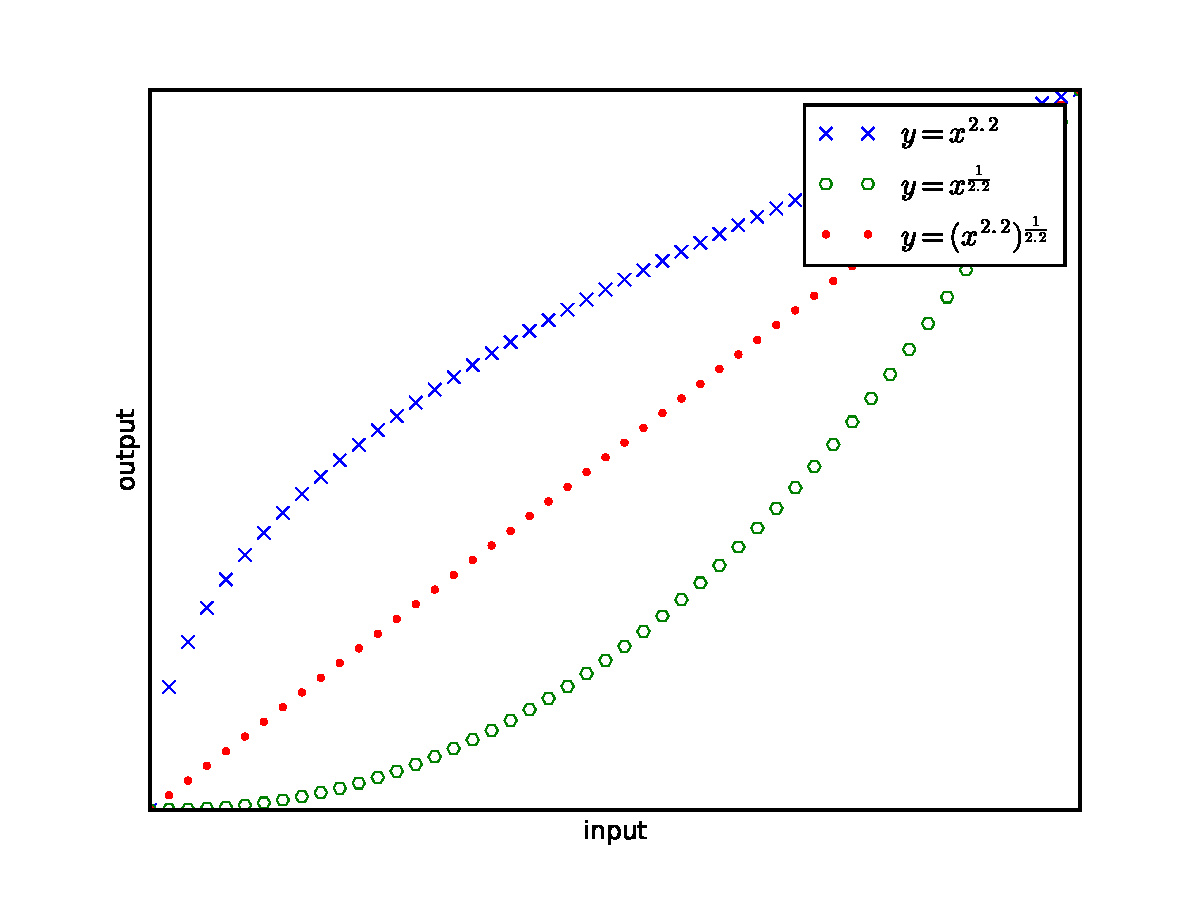
\includegraphics[width=0.5\textwidth]{gamma_coding}
  \label{fig:gamma_coding}
  \caption{Gamma encoding and decoding functions, $\gamma = 2.2$}
\end{figure}

Asynchronous pixel behaviour is approximated via differencing the current image obtained by the camera and a reference frame; whenever a pixel's difference is larger than a certain threshold, we mark that position as ``spiked''. Each spike carries a flag, \textit{up} if there was a positive change in intensity or \textit{down} if a decrease was registered, this can also be thought of as a spike's \textit{sign}. Depending on the selected type of output we simulate a receiver and update the reference accordingly. This is the basic DVS emulation and it's illustrated in Figure~\ref{fig:dvs_emu}.

\begin{figure}[htb]
  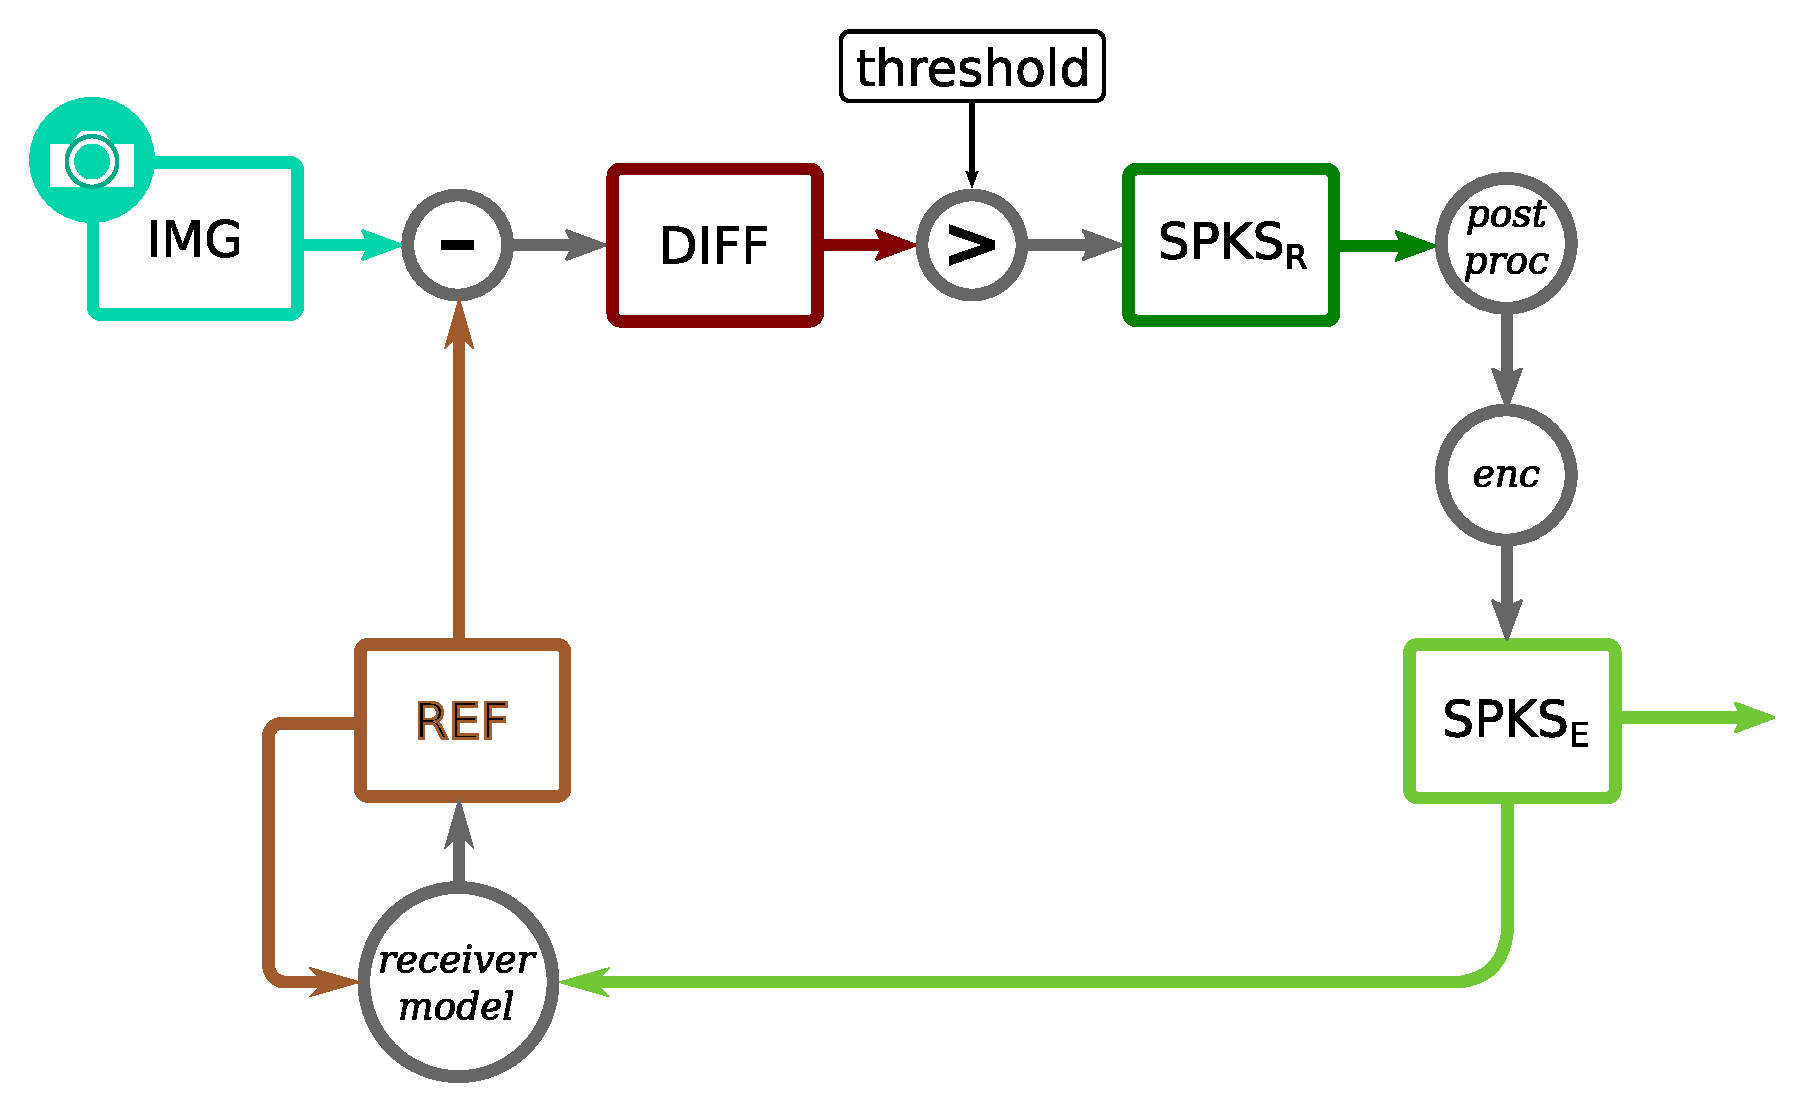
\includegraphics[width=0.5\textwidth]{dvs_emu}
  \label{fig:dvs_emu}
  \caption{DVS emulation diagram. Circles indicate operations and rectangles states of data}
\end{figure}

\subsection{Output modes}
\subsubsection{Rate-based}
As in previous emulators\cite{dvs_emu}, the standard output format is rate-based. In this mode each spike can be interpreted as an increment or decrement in intensity. To calculate the number of spikes that represents this change in intensity we use the following expression
\begin{equation}
  \label{eq:num_spikes_rate}
  N_{H} = \left\lfloor \mathrm{min}\left( T, \;\; \frac{\Delta I}{H} \right) \right\rfloor
\end{equation}
where $N_{H}$ is the number of spikes needed to represent the change in intensity $\Delta I$ in terms of the threshold $H$. Notice that the maximum time to transmit all the spikes for one frame is bound by the frame rate of the camera~$(fps)$. If it's only possible to send one spike per millisecond, we can send as many spikes as milliseconds in one frame-capture period ($T = 1000/fps$). At this stage we model a perfect receiver, so the quantity that will update the reference is
\begin{equation}
  \label{eq:ref_update}
  \Delta R = N_{s}\times H
\end{equation}

\subsubsection{Time-based}
In its worst case rate-based encoding can send a spike per millisecond per pixel, which can potentially saturate communication channels. One way to prevent this is to encode the value that each spike represents in the time each it is sent.

First we propose to linearly encode the number of thresholds exceeded. To do this the result of Equation~\ref{eq:num_spikes_rate} would in, a bin width $\left(W_{b}\right)$ of 1~ms was used for time discretization. As in the previous case the time to send all spikes for the current frame is at most $N_{b}=T/W_{b}$, which means the maximum difference possible is $T\cdot H$.

Figure~\ref{fig:linear_time} shows the value-to-spike-time relation, in our proposal earlier spikes represent larger changes in intensity. The main advantage of this encoding is that a single spike could represent multiple rate-based spikes, though the encoded values are limited by time resolution and the frame rate of the camera.

\begin{figure}[htb]
  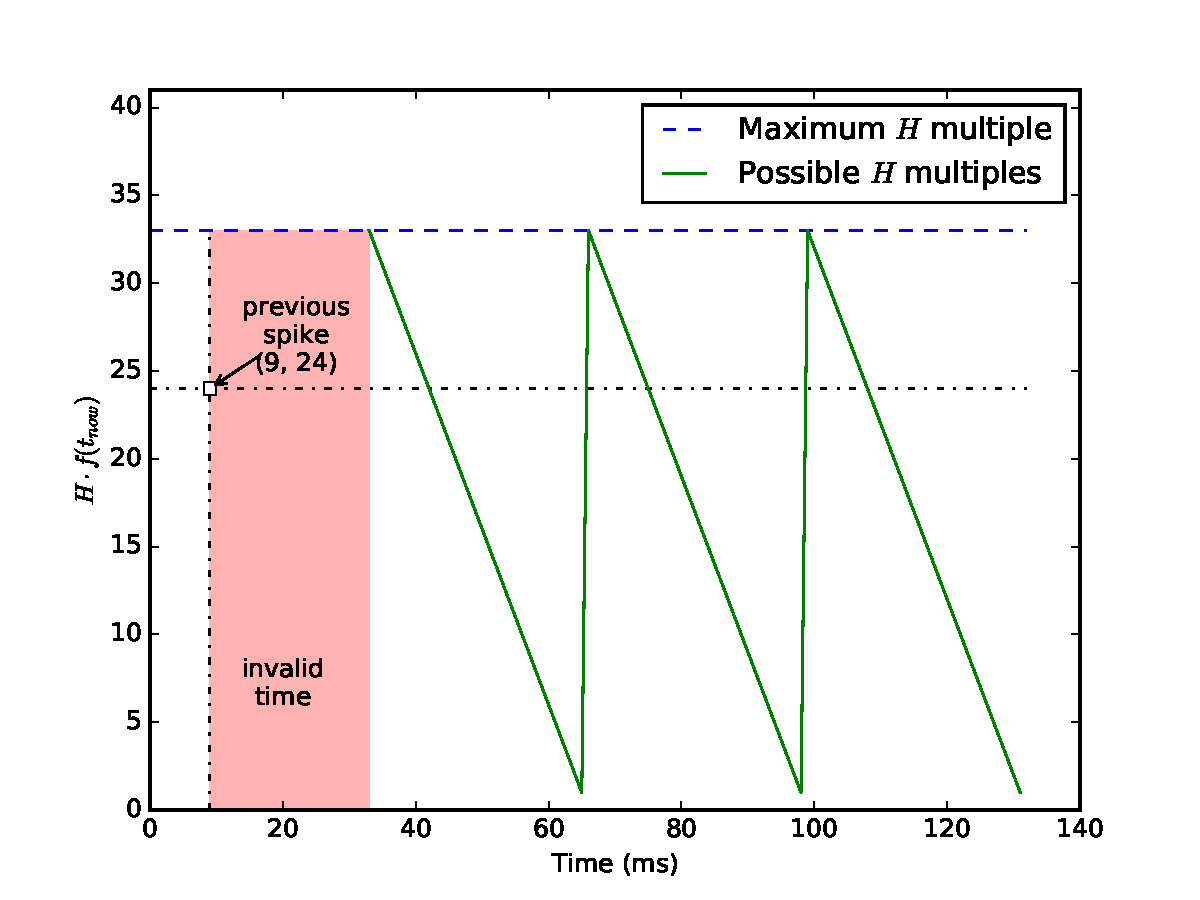
\includegraphics[width=0.5\textwidth]{spike_values_linear}
  \label{fig:linear_time}
  \caption{Linear time-based encoding of thresholds ($H$) exceeded}
\end{figure} 

To decode on the receiver end, we must keep track of the time and value from the last collected spiked. Let $\Delta t$ be the difference in arrival time between the previous and current spike~(Eq. \ref{eq:time_diff})

\begin{equation}
\Delta t = t_{now} - \left( t_{last} - N_{H}^{last}W_{b} \right)
\label{eq:time_diff}
\end{equation}
where the subtraction of $N_{H}^{last}W_{b}$ resets the time reference to a multiple of time period $T$. We now divide the time difference by the time-bin width to obtain the current bin
\begin{equation}
B = \frac{\mathrm{mod}\left(\Delta t, \;\; T\right)}{W_{b}}
\label{eq:bin_compute}
\end{equation}
here, $\mathrm{mod}$ calculates the arguments' division remainder. Now that the time bin $B$ is known, all it takes to compute the number of thresholds exceeded is
\begin{equation}
 N_{H}^{now} = \left\lfloor N_{b} - B \right\rfloor
 \label{eq:new_Nh_linear}
\end{equation}

%and reduce the probability of getting the wrong value
To overcome the limitation on maximum encoded values  we propose \textit{binary encoding} of either the absolute difference in intensity or the number of thresholds exceeded. The main advantage of this technique would be to achieve large values with fewer time bins as the growth is exponential (Fig. \ref{fig:exponential_time}). We propose to use this encoding in two ways: \textit{shoot-and-refine} and \textit{full value}. 

\begin{figure}[htb]
  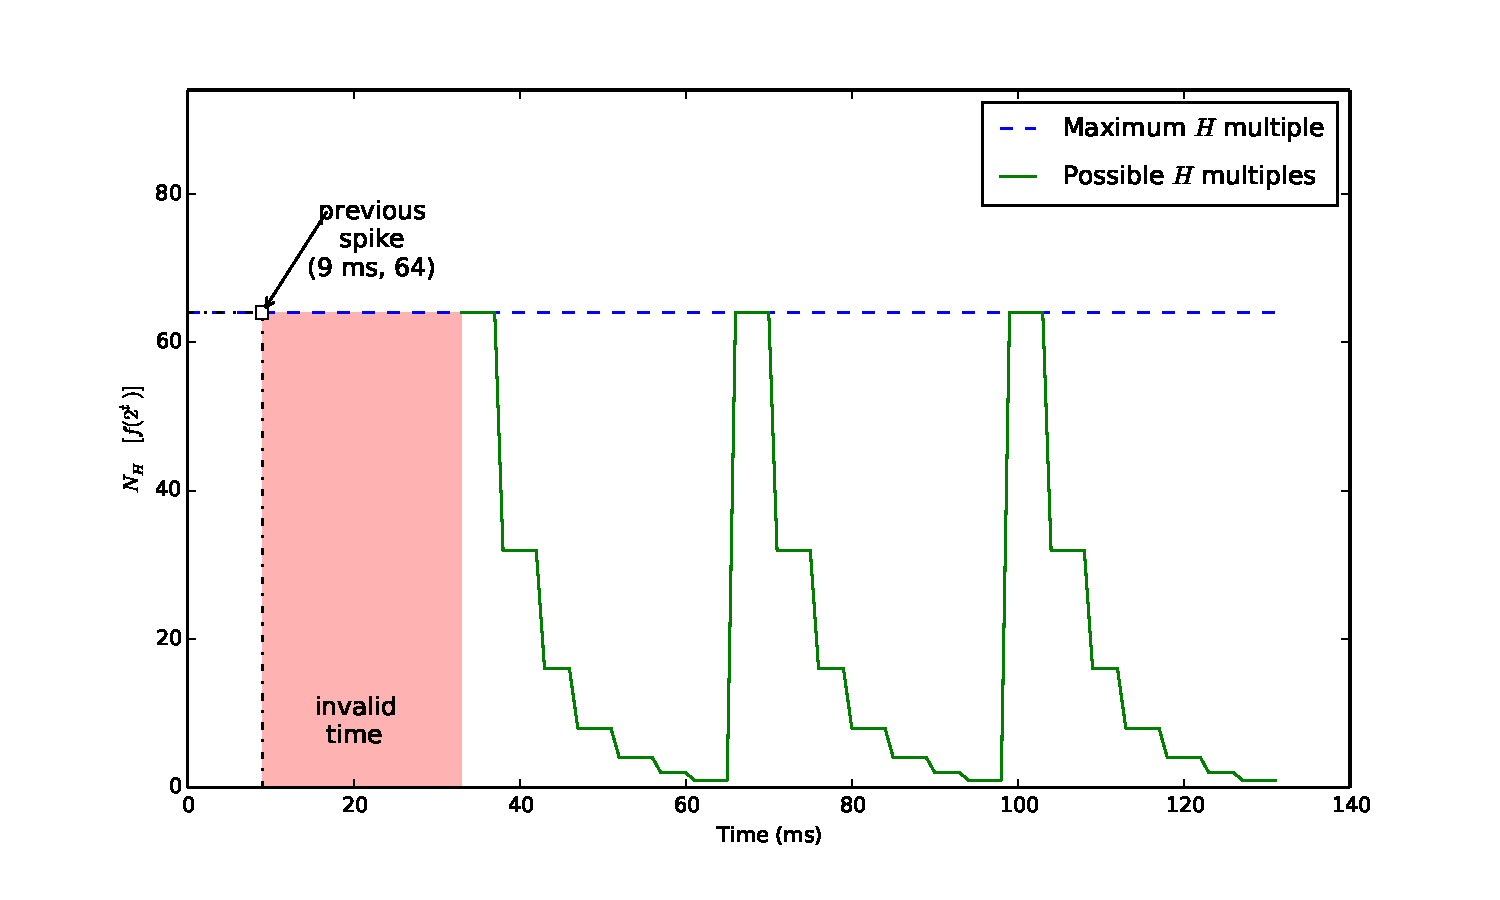
\includegraphics[width=0.5\textwidth]{spike_values_exp}
  \label{fig:exponential_time}
  \caption{Exponential time-based encoding of thresholds ($H$) exceeded}
\end{figure} 

In the \textit{shoot-and-refine} mode, a single spike is sent with an over- or underestimate of the desired value (e.g. the next power of two), and in the following frames we send at most one spike to refine the received value towards the desired one. Decoding can be done in a similar way as the linear case, but we divide the available time in $N_{b}$ bins of width is $W_{b} = T/N_{b}$. Now to compute the time difference
\begin{equation}
\Delta t = t_{now} - \left( t_{last} - log_{2}(N_{H}^{last})W_{b} \right)
\label{eq:time_diff_exp}
\end{equation}
and the right bin is calculated as in Eq.~\ref{eq:bin_compute}, finally for the decoded value
\begin{equation}
N_{H}^{now} = 2^{ \left\lfloor N_{b} - B \right\rfloor }
\label{eq:new_Nh_exp}
\end{equation}

For the \textit{full value} mode many spikes would be sent per pixel each frame, thus providing better resolution to the sent value, the downside to this is that an accumulation buffer is needed in addition to the previous spike time and value buffers. Decoding multiple spikes per frame has to be split in two cases: first if the new spike arrives before the current period is finished, then we accumulate its value to the current decoded value; otherwise we replace the contents of the accumulation buffer with the newly decoded value.

\subsubsection{What if spikes get lost?}

Initially we described a system where every spike that is sent will be captured on the receiver end, but this is not always the case. To cope with the latter cases, we now introduce a history decay mechanism which will allow the receiver to, in the long term, recover from missing spikes. 

\begin{figure}[htb]
  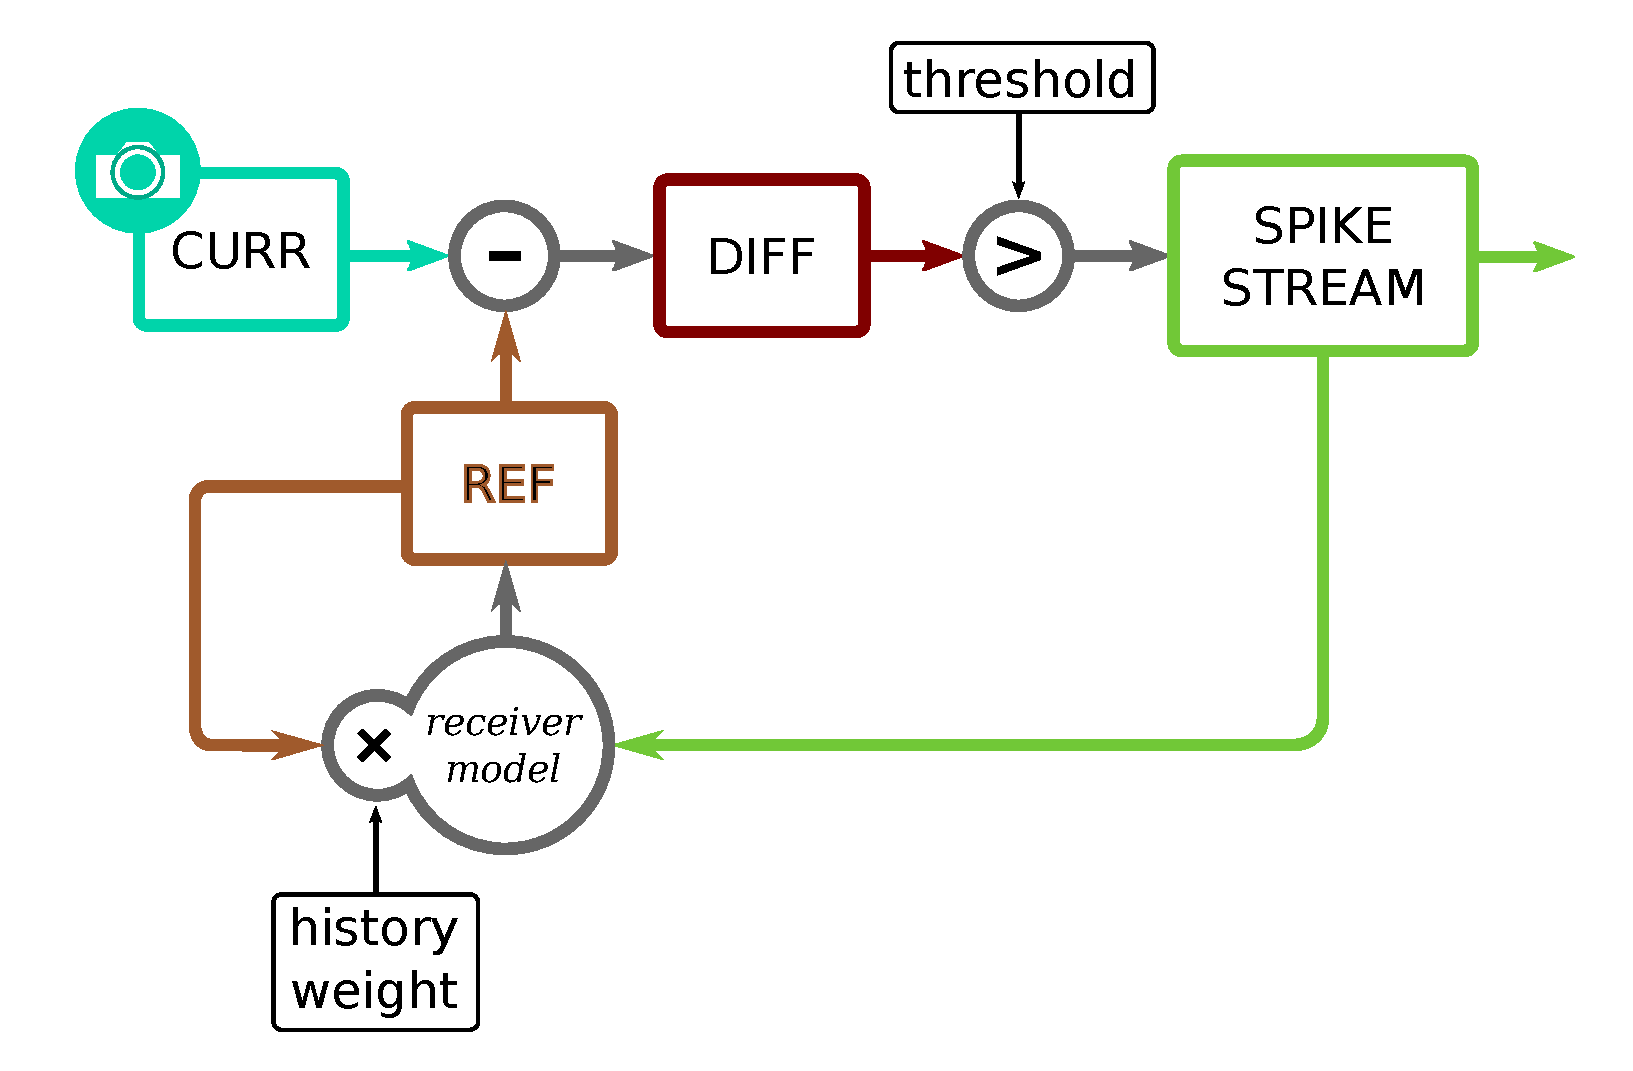
\includegraphics[width=0.5\textwidth]{dvs_emu_decay}
  \label{fig:dvs_emu_decay}
  \caption{DVS emulation with history decay. Circles indicate operations and rectangles states of data}
\end{figure}

\subsection{Additional behaviours}
\subsubsection{Local inhibition} reduces bandwidth, persistence of spatial stimuli over frames. 
\subsubsection{Adaptive threshold} slow-charging pixels by reducing the threshold.\\
Less parameters to configure.
\subsubsection{History decay}
Open source, and available in github.com\\

\section{Results}

Real-time DVS emulation on consumer hardware (Intel i5, 8GB ram)
sPyNNaker wrapper for videos and images.

\section{Conclusion}

GPU computing version would allow for higher resolutions.

Working on ganglion cell/Difference of Gaussian encoding.

\printbibliography
%\end{multicols}
\end{document}
